\documentclass{scrartcl}
\usepackage[utf8]{inputenc}
\usepackage[UKenglish]{babel}
\usepackage{caption}
\usepackage{listings}
\usepackage{pdfpages}
\usepackage{amsmath,amssymb}

\newcommand{\qed}{\hfill $\blacksquare$}

\lstset{frame=single,keepspaces=true,captionpos=b}

\title{Homework 04 - Linear Regression}
\author{Arne Sachtler - \textit{Registration Number: 03692662}}
\date{\today}
\subtitle{IN2064 Machine Learning}

\begin{document}
\maketitle

\section{Least Squares Regression}

\subsection{Problem 1}

See the generate pages in appendix~\ref{app:nb}.

\subsection{Problem 2}

Given loss function:
\begin{equation}
	E_{weighted}(\mathbf{w}) = \frac{1}{2} \sum_{i=1}^{N} t_i \left[\mathbf{w}^\top \mathbf{\phi}(\mathbf{x}_i) - y_i\right]^2 \, .
\end{equation}

Introduction of a diagonal matrix $\mathbf{T}$ with the weights $t_i$ on its diagonal enables one to rewrite the given loss function in full matrix notation with the design matrix $\mathbf{\Phi}$ and the full vector of target values $\mathbf{y}$. This yields
\begin{eqnarray}\label{tt}
	E_{w}(\mathbf{w})&=&\frac{1}{2} \left(\mathbf{\Phi}\mathbf{w} - \mathbf{y}\right)^\top \mathbf{T} \left(\mathbf{\Phi \mathbf{w} - \mathbf{y}}\right) \\
	&=& \frac{1}{2}\left(\mathbf{w}^\top \mathbf{\Phi}^\top \mathbf{T} \mathbf{\Phi} \mathbf{w} - 2 \left(\mathbf{y}^\top \mathbf{T} \mathbf{\Phi} \mathbf{w}\right) + \mathbf{y}^\top \mathbf{T} \mathbf{y}\right) \, ,
\end{eqnarray}
where
\begin{equation}
	\mathbf{T} = \begin{pmatrix}
		t_1&&\ldots&0\\&t_2&&\vdots\\\vdots&&\ddots&\\0&\ldots&&t_n
	\end{pmatrix} \, .
\end{equation}

Computing the derivative with respect to $\mathbf{w}$ yields
\begin{equation}
	\frac{\partial E_w}{\partial \mathbf{w}} = \left(\mathbf{\Phi}^\top \mathbf{T} \mathbf{\Phi} \mathbf{w} - \mathbf{y}^\top \mathbf{T} \mathbf{\Phi}\right) \, .
\end{equation}
And consequently is follows that
\begin{equation}
	\hat{\mathbf{w}} = \left(\mathbf{\Phi}^\top \mathbf{T} \mathbf{\Phi}\right)^{-1} \mathbf{\Phi}^\top \mathbf{T} \mathbf{y} \, .
\end{equation}

The parameters $t_i$ act like a precision factor in the expression. Inspecting equation~\ref{tt} reveals that the matrix of weights $\mathbf{T}$ acts like the inverse of a covariance matrix in a multinomial normal distribution. We can see that $\mathbf{T}$ is comparable to $\mathbf{\Sigma}^{-1}$.

\section{Ridge Regression}
\subsection{Problem 3}
Ordinary linear least squares finds the minimum of the loss function
\begin{equation}
	E = \frac{1}{2} \left(\mathbf{\Phi}\mathbf{w} - \mathbf{y}\right)^\top \left(\mathbf{\Phi}\mathbf{w} - \mathbf{y}\right) \, .
\end{equation}

Using the augmented data set matrices as
\begin{equation}
	\mathbf{\Psi} = \begin{pmatrix}
		\mathbf{\Phi}\\\sqrt{\lambda} \mathbf{I}_M	
	\end{pmatrix} \quad \text{and} \quad \mathbf{z} = \begin{pmatrix}
		\mathbf{y}\\\mathbf{0}_M
	\end{pmatrix}
\end{equation}
and evaluated the loss function for ordinary least squared with these yields
\begin{eqnarray}
	E&=&\frac{1}{2} \left(\mathbf{\Psi}\mathbf{w} - \mathbf{z}\right)^\top \left(\mathbf{\Psi}\mathbf{w} - \mathbf{z}\right)\\
	&=&\frac{1}{2} \left(\begin{pmatrix}
		\mathbf{\Phi}\mathbf{w}\\\sqrt{\lambda}\mathbf{I}_M \mathbf{w}	
	\end{pmatrix} - \begin{pmatrix}
		\mathbf{y}\\\mathbf{0}_M
	\end{pmatrix}\right)^\top\left(\begin{pmatrix}
		\mathbf{\Phi}\mathbf{w}\\\sqrt{\lambda}\mathbf{I}_M \mathbf{w}	
	\end{pmatrix} - \begin{pmatrix}
		\mathbf{y}\\\mathbf{0}_M
	\end{pmatrix}\right)^\\
	&=& \frac{1}{2} \begin{pmatrix}
		\left(\mathbf{\Phi w}-\mathbf{y}\right)^\top & \sqrt{\lambda} \mathbf{w}^\top 
	\end{pmatrix} \begin{pmatrix}
		\left(\mathbf{\Phi w}-\mathbf{y}\right)^\top \\ \sqrt{\lambda} \mathbf{w}^\top 
	\end{pmatrix}\\
	&=& \frac{1}{2} \left(\mathbf{\Phi}\mathbf{w} - \mathbf{y}\right)^\top \left(\mathbf{\Phi}\mathbf{w} - \mathbf{y}\right) + \frac{1}{2} \lambda \mathbf{w^\top w} \, ,
\end{eqnarray}
which is exactly the same loss function as that solved by ridge regression. \qed
\pagebreak
\appendix
\section{Notebook for the Linear Regression Task}\label{app:nb}
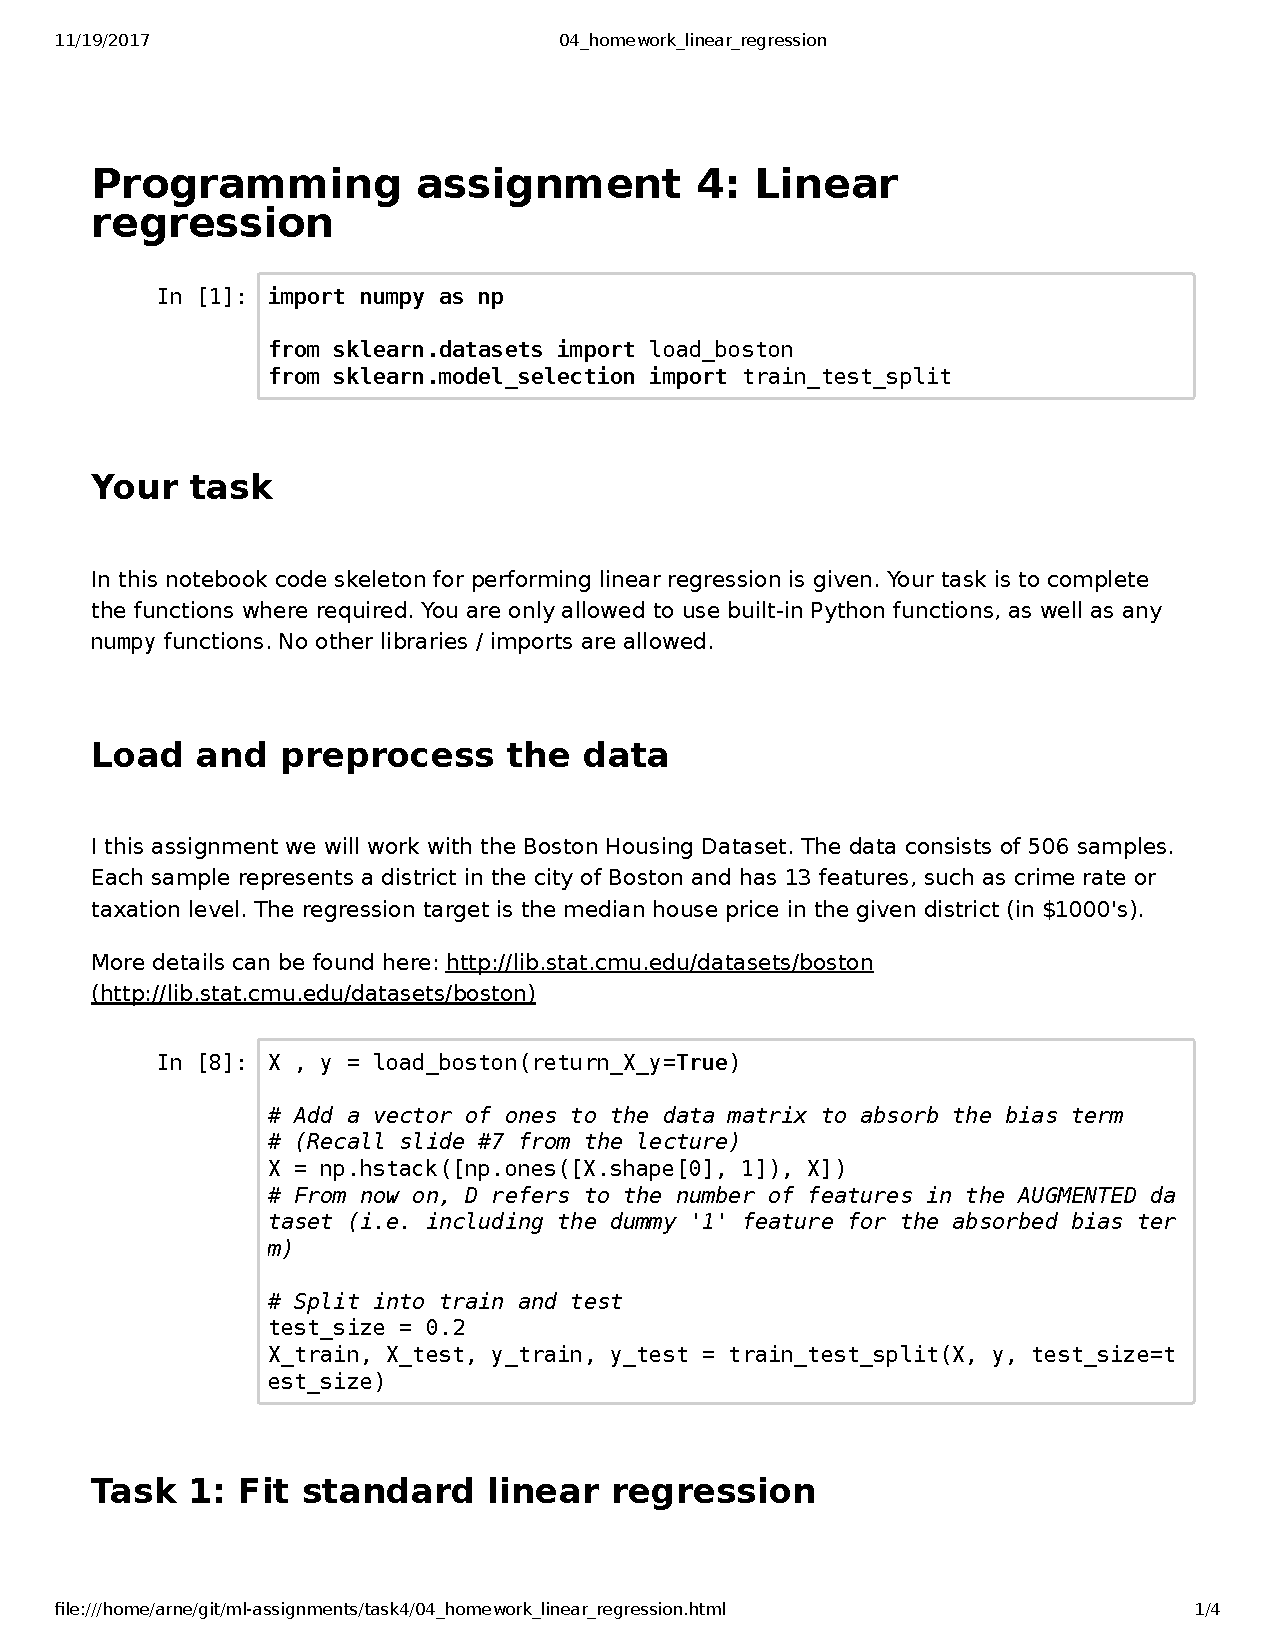
\includepdf[pages=-]{../04_homework_linear_regression.pdf}

	
\end{document}